
\section{Knowledge Management}
\label{sec:km}

Software development is inherently a knowledge-intensive activity. Software
designers and developers leverage their software-development skills, along with
domain knowledge, past experiences, and the knowledge of team members, to solve
the problem at hand, such as implementing a new feature or resolving a bug.  In
small, collocated teams, knowledge management is not a big challenge---people's
expertise on different parts of a system is typically known. New team members
can use informal communication channels to identify experts and seek their help
as needed.

However, as teams increase in size or become geographically distributed,
knowledge management starts to become challenging. In large or distributed
teams, system knowledge---\eg expertise, dependencies, best practices---is
spread across multiple people, locations, and (in the case of outsourcing) even
organizations~\cite{Desouza:2006}. In such projects, a knowledge-management
system is needed to create \textit{project memories} that can serve different
needs. First, it should assist new team members in understanding the project
with little or no face-to-face guidance and identifying experts to reach out to
for questions. Second, the system should help existing team members identify the
artifacts relevant, and the people they might need to coordinate with, for
performing a task. Existing attempts at creating such project memories include
Hipikat~\cite{Murphy:2005} and Codebook~\cite{Begel:2010}.

A service company has a large, geographically distributed employee base, with
frequent employee churn at project and organization levels. To maintain
consistent delivery quality, it is essential to manage knowledge at the project
level. Moreover, because services is a price-sensitive business, there is also
the need to be cheaper and better, by doing more with fewer or less-skilled
resources. Driven by this need to gain competitive advantage in increasingly
competitive markets, it becomes essential for companies to build
\textit{organization memories} that store the collective knowledge of past
engagements, processes, and people to increase productivity and reduce
activities that ``reinvent the wheel.'' The intent behind such a system is to
ensure that the knowledge of past or current employees is available to other
employees when the need arises. Thus, the organization should be able to
leverage learning and solutions from past client engagements in the context of a
new similar engagement, even when members from the past projects are not around.

The need for organization-level knowledge bases is well established in the
management literature~\cite{davenport2000working,bollinger2001managing}. Equally well known is the fact that creating an
effective organization-wide knowledge base is very challenging~\cite{McKinsey:1999,Harvard:1999,Ernst:1997}. There
are challenges in: (1) \textit{knowledge creation}---how to codify explicit and
tacit knowledge and motivate individuals to contribute; (2) \textit{knowledge
  retrieval}---data versus information versus knowledge; (3) \textit{knowledge
  governance}---legitimacy, relevance, and quality of contributed
knowledge. Alavi and Leidner~\cite{Alavi:2001} present a good overview of
research issues in organization knowledge management. Prior research suggests
that IT is incapable of capturing organizational knowledge
\cite{malhotra2004knowledge,mcdermott2000information}, but also postulates that IT is the
strongest enabler for organization knowledge management systems (OKMS).

Next, we present three scenarios illustrating the need for OKMS in service
companies. Then, we discuss promising research directions based on our
experience with building systems intended to promote knowledge reuse in these
scenarios.

\subsection{Scenarios for OKMS}

In this section, we present three typical scenarios in service delivery that can
benefit from an organization knowledge management system.

\subsubsection{Troubleshooting}

One of the common forms of service engagements is application maintenance, where
the expectation from the service provider is to take over a client's custom
application and handle service requests for it.  Service requests come in the
form of trouble ``tickets'': users of the applications can raise a ticket,
logging a problem they have experienced. This is similar to defect logging in
bug repositories, such as Bugzilla, where users of an open-source software can
enter the details of a problem that they encountered.  The main difference is
that, in typical software development in open-source communities, there is no
obligation on the development team to address the defects in a timely
fashion. Likewise, even in a product setting, the development team can
prioritize which defects they are going to address first.  In service context,
the service provider is supposed to resolve the ticket in a timely manner, often
under a service-level agreement. For example, a critical bug must be resolved
within 6~hours, at risk of financial consequences for the provider.

Software development in service organizations is not pure custom
implementations. In many cases, packaged applications, such as SAP, Oracle, and
COTS products, with client-specific customizations and external libraries are
used. The cause of a problem ticket could be in the customization done for the
client, in the way external code is used, or even a bug in the external code. If
the issue is with the configuration or the external code, it is very likely that
the same (or a similar) issue has been resolved previously in the context of
another client. Thus, if the person attempting to resolve the current ticket had
access to previously resolved tickets addressing similar problems, they could be
much more efficient and effective at their task.  Therefore, a knowledge base
that stores past resolved tickets across clients would be a useful
organization-wide resource. 

In a way this knowledge base would be similar to question and answer forums we see on various software languages, tools, open source projects on the WWW. 

\subsubsection{Design-build Projects}

Another common form of service engagement is business-process transformation,
where the expectation from the service provider is to IT-enable a business
process, such as payroll management, vendor management, order-to-cash, for a
client. Some business processes (\eg payroll management) would be required by
all clients, whereas other processes would be common in a particular domain (\eg
claim-management process in the insurance domain).  The client expectation is
that the service provider possesses adequate knowledge of the generic version of
a particular process, creates client-specific variations, and implements the
system. Typically, this requires that the vendor team working on the project has
significant domain experience.

A knowledge-management system that stores past business process implementations
across the organization can help in this scenario. The past solutions need to be
organized by domain to make retrieval of relevant information
easier. Appropriate documentation that explains the standard and customized
portions of past solutions needs to be available, along with the solution
code. While designing a new business-process solution, the team can search
through the repository to learn about the variations of the process to be
implemented and, if the client requirements are not too different from a past
solution, even reuse the solution in totality or parts. This can reduce the
overall cost and also potentially let the service provider staff the team with
people with less domain experience. 

Code reuse has been an area of interest to software engineering community, be it reuse of a couple of code lines, API use or even complete solutions \cite{Reiss:2009,Holmes:2013}. Much of this work can be applied in an services organization setting too.

\subsubsection{Service Improvement}

When a client outsources its application maintanence to another organization,
one of the key expectations is that the vendor would bring down their total cost
of ownership over time. This requires the vendor to proactively seek out areas
for improvement in the client application portfolio. One way to determine
whether there is scope of improvement in an application in the client IT
landscape is by benchmarking its performance against other similar applications
in other client landscapes. To illustrate, suppose that a service company
maintains the payroll applications for 10~clients. For nine of the clients, the
monthly ticket volumes range between 5 and 10 tickets, whereas, for the
remaining client (say client~A), the ticket volume ranges from 20 to 50. This
indicates that, for client~A, investigations could be conducted to determine the
root causes for high ticket volumes and appropriate preventive actions
taken. Moreover, if a similar high-ticket-volume problem was seen in the past in
another client's payroll system, information about the actions taken for that
client could help the team resolve the problem for client~A.

There are a number of organizations that gather and report quantitative benchmark information (qualitiative as well as productivity) for software projects and business applications depending on language used to code, number of users etc. CAST, Software Engineering Institute are some examples of such organizations. However, considering services organizations are doing multiple software implementations for multiple clients, an organization-wide knowledge base that (1) captures key
operational metrics per application (or at a more granular level, such as by
problem area) per client and the past improvement actions taken, and (2) allows
comparisons between clients with similar applications and problems encountered,
would help augment what is publicly available and be more useful.


\begin{figure*}
	\center
	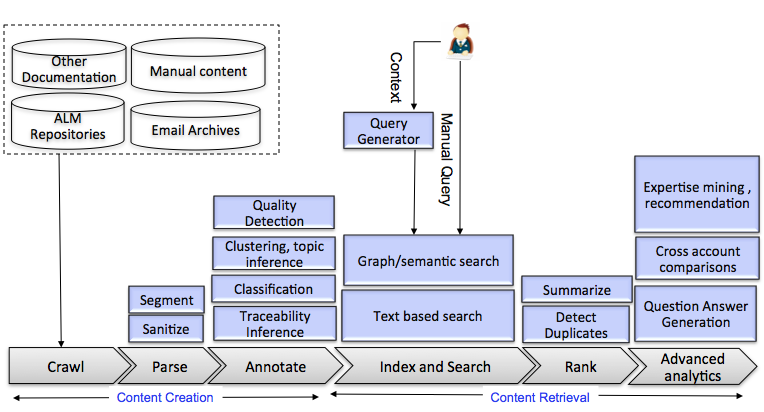
\includegraphics[scale=0.45]{figs/km.png}
        \vspace*{-10pt}
	\caption{System architecture for an OKMS system for a service company.}
        \vspace*{-10pt}
	\label{fig-km}
\end{figure*}


\subsection{Research Areas}

We encountered the above OKMS needs in IBM services division and made an attempt at building systems that addressed these needs. \cite{Majumdar:2011} describes a system that is in use in IBM that enables cross-account sharing of knowledge in problem tickets. \cite{Goodwin:2012b} discusses the system that was built to promote solution reuse in design-build engagements centered around business process transformation. We now outline some core problems that need to be addressed to create OKMS systems in services organizations. At the simplest level, a OKMS system is a database where content can be put and retrieved. However, what content should be put, how easily can it be put and further the ease with which relevant content can be retrieved determines whether the knowledge management system would be used or not. 
Figure ~\ref{fig-km} shows the advanced the architecture for an OKMS system in services. The blue boxes indicate areas that could benefit from further research. 

\subsubsection{Content Creation}

The first challenge in building an OKMS system is identifying what data should be put in the repository and how to obtain the data. An organization has the option of mandating that each of it's employees contributes their learnings to the OKMS system. Some examples of manual knowledge creations are: (1) frequently asked question, where employee outlines the typical solutions to some common problem tickets they have resolved (2) postmortem reports, usage stories, experience reports\cite{desouza:2005}, that project members can create after they solve a key issue in the project. To enable solution reuse, services organizations often invest in creating software product families \cite{clements2002software}. However, here it's pre-anticipated what could be some solutions that could be of interest to multiple clients in a particular domain such as healthcare and then those solutions are created with appropriate points for variability built in, so solution can be customized for any client intending to use it.  Once a project is completed, employees are also encouraged to identify reusable components in software they created and share them in the knowledge base. This approach of manual content creation adds extra burden on the employees. An open research challenge is to motivate employees to contribute high quality content in the knowledge base \cite{hendriks1999share}. Open source forums such as stack exchange have experimented with elaborate incentive mechanisms in forms of badges to ensure questions and answer contributions on their forums \cite{vasilescu2014social}. In services organizations are reputation building incentives enough or incentives should translate to monetory benefits and/or career progression /cite{bartol2002encouraging}? 

Another approach for content creation is to auto-harvest artifacts produced in the SDLC lifecycle and put these in the knowledge management system. Complete traceability from requirement through code to test cases, along with their content is extractable from Application Lifecycle Management tools and this can act as solution packs to put in the repository. Similarly for ticket resolution, information about problem ticket and it's resolution is extractable from ticket management systems. Account teams periodically report on various important metrics on the applications being maintained in the client landscape such as ticket volumes, code changes, service improvement actions taken. These reports can be auto pushed into the knowledge repository. The main challenge here is crawling and parsing of this data from various tools and work product templates being used across clients and collating this information into a standardized format that can be pushed into the knowledge repository. Many of this work products are documents in proprietery formats such as Microsoft word, power point slides, visio diagrams, excel sheets. How to automate content extraction from client specific work products into the standard format used by knowledge repository is again a direction for research. One approach is to write model to model transforms where a project admin can specify the mapping \cite{debdoot:2010:scc}. Another challenge is that requisite traceability information that is required to understand complete context of how and why an artifact was produced, might be missing. This is because tools being used to create different SDLC artifacts have not been integrated. There is need to auto infer traceability between artifacts
For example, if making a code commit, the developer puts in a comment like "Fixed Bug \#145", then with high confidence the change is to fix "Bug \#145" and traceability edge between code file and bug report should be auto-created. 
. Tracability inference is an active area of research \cite{spanoudakis2005software}. Some proposed approaches use information retrieval (IR) techniques, others use traceability rules, special integrators, and inference axioms.


The content put in the OKMS should be organized in such a way that retrieval becomes easier when someone needs it. The general practice is to classify OKMS content against pre-defined taxonomies. One taxonomy is obviously the object type i.e. requirement, code, problem ticket (further segmented into problem description, resolution). Another taxonomy captures the domain the artifact was produced in i.e. industry type and process area e.g. \cite{apqc,bph}. Another taxonomy is the technology used. Organizations spend effort building and maintaining these taxonomies. For every data that is put into the knowledge base, the content needs to be manually categorized against these pre-defined taxonomies. Pattern matching and machine learning based classification approaches /cite{bishop2006pattern} can be used to auto-categorize content to these pre-defined taxonomies. These techniques rely on the availability of equal proportion of positive and negative samples to train a learning model. However, due to unavailability of training data and/or lack of differentiating features, usual learning techniques such as naive bayes, support vector machines, decision trees, might end up not giving desired efficacy (measured as precision and recall). There is need to customize more advanced learning approaches such as adaptive learning, ensemble techniques or develop new techniques that work well with SDLC data. Another interesting area for research is to explore how to help grow the taxonomy over time based on content coming in the knowledge base. Techniques such as clustering \cite{Berkhin06}, topic modeling \cite{Blei:2012} help group together similar looking content and infer topics out of them. 

The content in a OKMS database comes from various client projects. There are strict privacy constraints around what data is client confidential and hence cannot be shared. Within a single artifact itself, there might be small portions of content that are client confidential. E.g. a problem ticket might content the contact information of the user who encountered the information. How to remove client confidential data from artifacts put in the repository, how to anonimize the content so as to not disclose client identity and how to ensure that only authorized users and roles have access.

Once an OKMS system is implemented in an organization, irrespective of the approach to collect content i.e. manual, automated harvesting or hybrid, the repository starts filling up fast. Over a period of one year, the problem ticket repository we setup within IBM collected 750K tickets. Similarly, the business process solution repository has 16000 solutions. However, not all content being put in the repository is high quality and reusable. Hence, it is becomes imperative to be able to filter out useless content. One way to achieve this is by making a human vet every content being pushed in the repository and only content that is deemed high quality is published. Another approach is to ask people who are retrieving and potentially using the content, give feedback on whether they found content useful or not. The third approach that makes for an interesting research direction is to explore how a an automatic quality score can be assiged to each artifact based on content in the artifact, prior reputation of people who authored the content, whether the project was a success or not and so on. In our problem ticket repository, we experimented with calculating a quality score per ticket based on technical versus non-technical content present in the ticket \cite{Majumdar:2011}.

To summarize, content creation in OKMS provides multiple oppurtunities where research can contribute. These include: what and how to extract content from SDLC repositories and proprietry document formats, how to infer traceability between different artifacts, how to classify and categorize content, how to maintain privacy, estimate quality and motivate employees to contribute high quality content. 

\subsubsection{Content Retrieval}

A good OKMS system is one that not only had good content, but one that makes it easy to retrieve the content when needed. Typical ways to retrieve content from a knowledge base are: (1) keyword based search where user specifies a couple of words (s)he is looking for and all artifacts in the repository that contain the words from user query are returned, (2) faceted (or navigational) search where user is shown a hierarchy structure (taxonomy) and can browse information by choosing one or more values from each of the pre-defined categories. Various language based information retrieval models \cite{manning2008introduction} such as vector space models, probablistic models, latent semantic index exist that can be used here. But inspite of easy to use search technologies being available, prior studies report that knowledge retrieval from organization wide repositories remains a challenge. As per \cite{idc,idc2}, while employees spend 15\% to 35\% of their time searching for information in an enterprise, they are successful less than 50\% of the time in finding what they are looking for. 

Non-availability of content or poorly organized content can be one reason for this. Another reason could be the inadequacy of the query itself that are used to retrive the content. Suppose a user is trying to find problem tickets that resolved similar issues to what (s)he has been assigned. (S)he would pick up a couple of words from the ticket that describe the problem and use it to query the knowledge base. However, these words might not be discriminative enough and user might end up getting too many or too little search hits. Another approach could be to use complete content in the ticket and use it as query. However in this case, the search engine might end up returning irrelevant results as equal weightage was given to all words in the problem ticket. \cite{Sinha:2012} tries to address this issue by giving more weightage to those words in the query that belong to ticket title. \cite{Ashok:2009} parses out different datatypes from a problem ticket such as description, application information, stack trace and using a different query/search mechanism for each. E.g. instead of just specifying "null pointer exception", the query generated from a problem ticket could be---description: contains following bag of words \{null, pointer, exception\}, process: is equal to "order to cash", stack trace: contains foo.*bar. The results obtained from such a query are likely to be more precise than what a keyword search would yield. A challenge with this approach is how to compose the various clauses in the query---are they "anded" or "ored" or a combination. Another challenge is how much weightage to give to each clause when ranking the search results \cite{Debdoot:2011:bpm}. Moreover, recently contextual search \cite{wen2004probabilistic,kraft2005q} has been gaining momentum. Contextual search tries to better capture a user's information need by augmenting the query with contextual information extracted from search context. It would be an interesting direction for future research to see for each of the knowledge needs in services organizations, what can make up the context, how to use this context to create the query and how to weigh different clauses in the query. 

Any search based system would return multiple results. For the user it becomes a chore in itself to go over each of the search results and identify if it is relevant or not. Techniques that can help the user easily comprehend the relevance of the returned results are much needed. Text based search engines highlight the matching words between query and content of the artifact returned. However, when the query becomes complex (as above), keyword highlighting is not of much help. In text processing domain, summarization is one approach that is used to help end users get a quick idea of what the content is about. In \cite{Mani:2012,Rastkar:2010} authors present different techniques to summarize bug reports. Research can help in developing summarization techniques that work for other SDLC artifact such as code, requirements, solution design documents and so on. Further, out of the search results returned many artifacts could be duplicates or near duplicates of each other. In order to reduce information overload for end user, the OKMS system should be able to group together duplicates and near duplicates and be able to highlight the variances in seemingly similar artifacts returned in the search results. Duplicate bug report detection \cite{wang2008approach,sun2010discriminative} has been a widely researched topic. Similarly for each of the artifact of interest from a services OKMS perspective, a customized duplicate detection approach might be needed. 

Most existing OKMS systems use language based IR models to store and retrieve knowledge. However, as we saw in content creation section, the repository is not just a collection of artifacts but a network of linked artifacts. Use of graph databases for data storage and retrieval techniques such as semantic search techniques \cite{Guha:2003} or optimizing keyword search for graphs \cite{kacholia2005bidirectional}, are worth exploring.

OKMS today stops at providing search capabilities. Given a user query, the system returns back matching artifacts but makes no attempt at making any deductions. Consider the scenario of troubleshooting. A user is searching through the past resolved ticket repository to see if similar issues were resolved. There are multiple reasons why the issues could have arisen. Based on past tickets, the user needs to come up with potential hypothesis of why the issue could be arising and based on conditions (s)he is seeing in the current landscape decide what hypothesis is applicable and then pick the appropriate solution. From such a user's perspective the OKMS system would be more effective if it were able to auto-generate these potential root causes and solutions hypothesis. Consider the service improvement use case, the accout team needs support from OKMS to identify similar projects, then compare the problems seen in the current project with different kind of issues arising in similar projects, then judge whether current team is doing better or worse and then decide to take some action. What kind of capabilities are needed in OKMS system to be useful in above scenarios is another area for research. 

There are two techniques for organization knowledge management, codification or personalization \cite{hansen2000s}.
Till now what we have discussed is what is called codification. Here knowledge is carefully captured and stored in the database, where it can be accessed and used by anyone in the company. This strategy allows many people to search for and retrieve knowledge without having to contact the person who originally developed it. This opens up the possibility of achieving required scale in knowledge reuse in services organizations. Another strategy for knowledge management is personalization. Here knowledge is  tied to person who developed is and is shared mainly through direct person-to-person contacts. The chief purpose of knowledge management system here is to help people find and connect to other people who have requisite knowledge, not to store it. This strategy works well when knowledge cannot be codified especially knowledge required to handle situations that require complex decision making. Expertise browser \cite{Mockus:2002}, expertise recommender \cite{McDonald:2000} have attempted to identify experts on various topics within a project. \cite{Balog:2006} has explored expertise mining and recommendation in predominantly document based OKMS systems. What information to use to mine expertise when repository contains SDLC data from multiple projects, how to match your current context and job profile to suggest people you should have in your network is another scenario where research can help. 

To summarize, content retrieval in OKMS system provides open research problems in query generation and use of context to augment queries, search result summarization, duplicate detection, use of semantic search to improve search relevance. Further the retrieval capabilities need to move beyond just search to provide capabilities such as question-answer generation, cross-account comparison/benchmarking and expertise recommendation.

